\section{Methodology} \label{sec:methodology}
% detailing the approaches that were used in your experiments; this may also include implementation details in relation to the mobile architecture used
According to \cite{sample_ref}, lorem ipsum dolor sit amet, consetetur sadipscing elitr, sed diam nonumy eirmod tempor invidunt ut labore et dolore magna aliquyam erat, sed diam voluptua. At vero eos et accusam et justo duo dolores et ea rebum. Stet clita kasd gubergren, no sea takimata sanctus est Lorem ipsum dolor sit amet. Lorem ipsum dolor sit amet, consetetur sadipscing elitr, sed diam nonumy eirmod tempor invidunt ut labore et dolore magna aliquyam erat, sed diam voluptua. At vero eos et accusam et justo duo dolores et ea rebum. Stet clita kasd gubergren, no sea takimata sanctus est Lorem ipsum dolor sit amet. Lorem ipsum dolor sit amet, consetetur sadipscing elitr, sed diam nonumy eirmod tempor invidunt ut labore et dolore magna aliquyam erat, sed diam voluptua. At vero eos et accusam et justo duo dolores et ea rebum. Stet clita kasd gubergren, no sea takimata sanctus est Lorem ipsum dolor sit amet.

\subsection{User Journey} \label{sec:user_journey}
Upon launching the soHappy app, the user will be presented with a home screen, where they can either start the app or navigate to miscellaneous screens via an options menu, in which the user may change settings, for example.
When the user starts the app, they will be asked to move their face into the camera frame. Until a face is recognized, a red tint is applied to the camera frame, providing visual feedback to the user. Advancing to different stages of the process changes the color of the tint accordingly.

Once a face has been detected, the red tint is changed to blue. At the same time, a countdown of three seconds is started, allowing the user to relax and take a couple of breaths.
After the countdown expires, a short text serving as a stimulus to smile is shown on the screen, prompting the user to recall memories they are fond of. A 30 second timer is started simultaneously, visualized as a growing progress bar at the top of the screen. Expiration of this timer causes the app to proceed to the next stage. An icon is displayed on the screen once a smile has been detected.
By virtue of the user seeing their own face during this process, genuine smiling may become difficult, especially if the user has problems with feelings of self-consciousness. In order to aid the user in smiling, a blur filter is applied to the camera, rendering objects harder to recognize.
Should the user fail to smile for at least ten seconds after their face has been detected, the process will be canceled. From this point, the user may opt to try again or continue on to the next part.

Following this process, a set of six questions querying current circumstances are posed to the user. Once all questions have been answered, the user will be thanked for their participation and presented with a percentage indicating how likely they are genuinely happy.

\subsection{Architecture}

The main goal of the software architecture of soHappy is providing flexibility 
in switching out various components.

Adding a Face or Smile Detector based on the technology of liking requires a
developer to implement the designated interface. The implementation can then be 
selected by modifying a configuration file of the app. A factory will create 
the Face or Smile Detector based on a configuration file. 

The image analyzer uses the created implementations of Face and Smile
Detectors. The results of the image analyzer are collected and stored in a
local database.

In order to load and manage the configuration file, a configuration manager 
is used.

Figure \ref{fig:arch1} shows the class diagram of the architecture.

\begin{figure}
    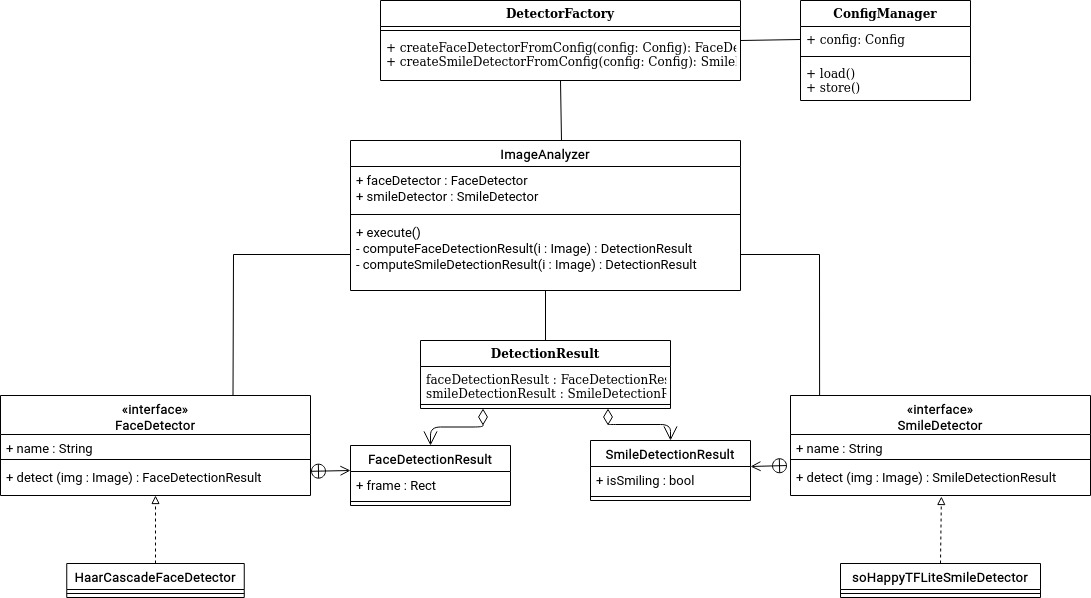
\includegraphics[width=\linewidth]{figures/methodology_architecture_1.jpg}
    \caption{Class diagram describing the architecture}
    \label{fig:arch1}
\end{figure}

On order to seperate to back-end logic from the User Interface, soHappy uses
``model-view-viewmodel'', a variant of the ``model-view-controller'' design 
pattern. The view is seperated by the model by the so called viewmodel, which
allows easy databinding to the UI (view), whilst allowing easy access from the
back-end (model). \cite{mvvm}

\subsection{State Machine}

\begin{figure}
  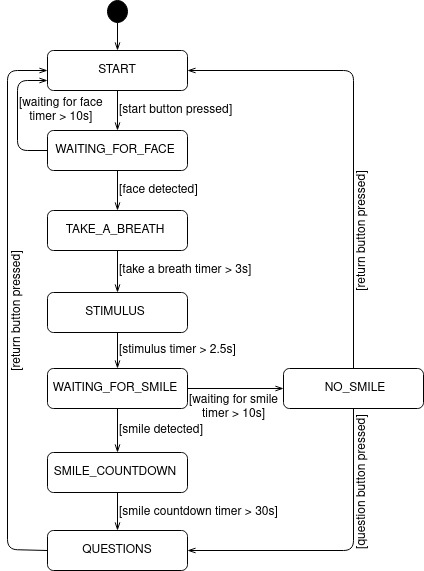
\includegraphics[width=\linewidth]{figures/state_chart.jpg}
  \caption{The state chart.}
  \label{fig:state_chart}
\end{figure}

State charts are used to describe the states and transitions of an state machine. A state is a situation in which an objects remains, until an certain event happens. Through such an impulse the state machine changed its state. Internal activities can be executed inside a state \cite{Modeling_with_UML}.

Figure \ref{fig:state_chart} shows the states and behavior of the applications state machine.
A state change can be invoked through three different kind of actions: An user action (for example pressing a button), a timeout after a specified timeframe or a significant analyser result (face detection or smile detection).

Note that if a face is detected and users move their faces out of the frame afterwards, the process continues and handles these event indirectly as missing smiles.
In addition, the face leaving the camera frame after a first smile detection is not dealt with explicitly but leads to low smile results.
Instead of having an end node, the application flow returns to the start screen, represented in the start state.

\subsection{User Interface} \label{sec:user_interface}
Like most smartphone applications, the soHappy app consists of multiple screens that the user can navigate through, each of them serving a different purpose. Such screens can be implemented in Android using the \texttt{Activity} and \texttt{Fragment} classes. An \texttt{Activity} object acts as an entry point to an Android app and provides a window for User Interface components to be created in \cite{intro_to_activities}. \texttt{Fragment} objects largely fulfill the same task, but are distinct from \texttt{Activity} objects in that they cannot persist on their own and must be hosted within an \texttt{Activity} object \cite{intro_to_fragments}. Since the soHappy app can only be started manually, a single \texttt{Activity} object for its sole entry point is sufficient. Each screen within the app is implemented with a \texttt{Fragment} object, which is hosted inside the single \texttt{Activity}. An example of how \texttt{Fragment} objects are implemented is shown in figure \ref{fig:user_interface}.

\begin{figure}
  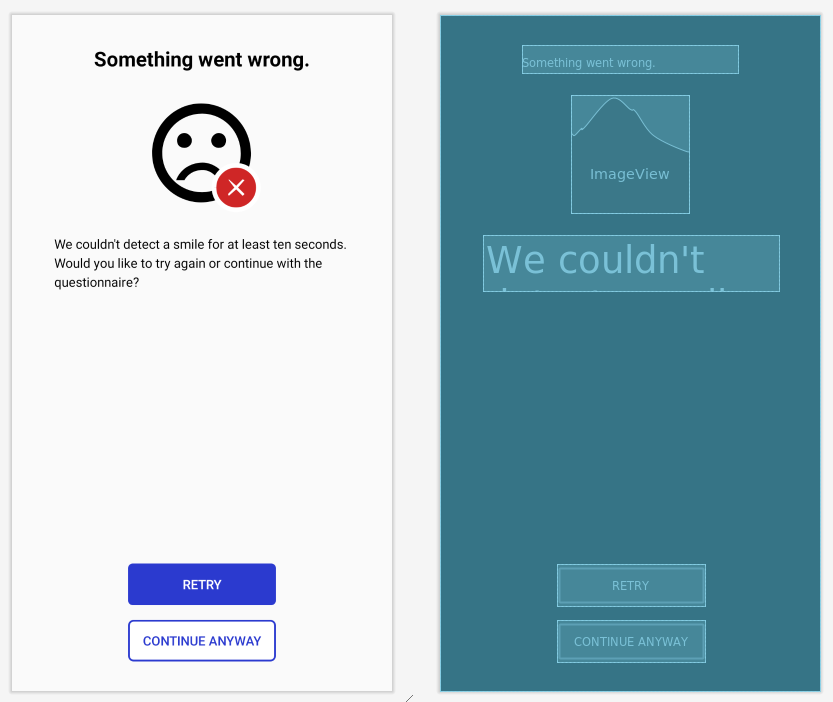
\includegraphics[width=\linewidth]{figures/user_interface.png}
  \caption{Example of a UI fragment designed in Android Studio's Layout Editor. A rendered screen is shown on the left, while its blueprint is depicted on the right.}
  \label{fig:user_interface}
\end{figure}

In terms of design, Android apps are generally expected to conform to Material Design, a set of guidelines defined by Google to help ensure both visual and practical consistency. As such, the user interface of the soHappy app is designed with Material Design in mind \cite{material_design}, incorporating principles such as animation or design based on the real world.

\subsection{Model Training}

As stated in the background section, soHappy uses a deep learning model to 
provide information about a person smiling by utilizing TFLite.

However, for TFLite to detect smiling, the model must be trained first. This
model is not trained on the device, but will be trained separately and shipped
with the android app.

The soHappy smile detection model is on based a convolutional neural network 
(CNN). CNNs are useful for image analysis purposes. A CNN utilizes multiple
convolutional layers as well as pooling layers. A convolutional layer works by
applying multiple different filters onto the input of the layer. A 
convolutional layer also looks at regions of the applied filter layers instead 
of individual pixels. This process is called convolution.
Pooling describes the process of discarding unused information.
Refer to \cite{8308186} for a more in-depth explanation on how CNNs work.

For the soHappy smile detection model, eight convolutional layers are used. 
Every two consecutive convolutional layers are followed by a pooling layer, 
repeated four times. In the end, a the result is flattened. This model
architecture is based on the work of Madnani \cite{MayurMadnani2018}.

In order to train the model, the dataset described in ``Smile detection using hybrid face representation'' \cite{Arigbabu2015} was utilized.
